\section{Background}

\subsection{Gaussian Process Regression}\label{sec:SOGP}

Given a training set $D_T = \{X, \bm{y}\}$ where $X = \{\bm{x}_1,~\dots~\bm{x}_N\}$, and $\bm{y} = \{y_1,~\dots~y_N\}$, we assume the target value $y$ is generated
by a latent function $f(\bm{x})$ with addictive noise $\epsilon \sim N(0, \sigma_n^2)$ such that
\begin{equation}
    \label{eq:yf}
    y_i = f(\bm{x}_i) + \epsilon_i.
\end{equation}
We use Gaussian process (GP)~\cite{GPML} to learn the latent function $f(\bm{x})$. A GP model defines a prior over $f(\bm{x})$. GP is fully characterized by a mean function $m(\bm{x})$ and a covariance function $k(\bm{x}, \bm{y})$. For the training set $D_T$, the latent function values $\bm{f} = (f(\bm{x}_1),~\dots~f(\bm{x}_N))^T$ follow a joint Gaussian distribution $\bm{f} \sim N(\bm{m}, K)$, where $\bm{m} = (m(\bm{x}_1),~\dots~,m(\bm{x}_N))^T$ is the mean vector, and $K_{ij} = k(\bm{x}_i, \bm{x}_j)$ is the covariance matrix. The mean function $m(\bm{x})$ can be any function, while the kernel function $k(\bm{x}, \bm{y})$ has to make sure that the covariance matrix is a symmetric positive definite (SPD) matrix. In this paper, we fix $m(\bm{x}) = 0$.

Given a new input $\bm{x}_*$, GP predicts the distribution of the output $y \sim N(\mu(\bm{x}_*), \sigma^2(\bm{x}_*))$, where $\mu(\bm{x}_*)$ and $\sigma^2(\bm{x}_*)$ can be expressed as

\begin{equation}
    \left\{
        \begin{array}{lll}
            \mu(\bm{x}_*)      &=& k(\bm{x}_*, X) (K + \sigma_n^2 I)^{-1} \bm{y} \\
            \sigma^2(\bm{x}_*) &=& \sigma_n^2 + k(\bm{x}_*, \bm{x}_*) - k(\bm{x}_*, X) (K + \sigma_n^2 I)^{-1} k(X, \bm{x}_*),
        \end{array}
    \right.
    \label{eq:GPRPred}
\end{equation}

where $k(\bm{x}_*, X) = (k(\bm{x}_*, \bm{x}_1),~\dots~,k(\bm{x}_*, \bm{x}_N))$ and $k(X, \bm{x}_*) = k(\bm{x}_*, X)^T$. In \eqref{eq:GPRPred}, the $\mu(\bm{x}_*)$ and $\sigma^2(\bm{x}_*)$ and be viewed as the prediction and the uncertainty measure.

There are usually some hyperparameters for a GP model, including the noise level $\sigma_n$ and the hyperparameters for the kernel functions. For example, the squared exponential kernel is a commonly used kernel in GP regression. The kernel function is defined as

\begin{equation}
    \label{eq:GaussianCovarianceFunction}
    k(\bm{x}_i, \bm{x}_j) = \sigma_f^2 \exp\Big(-\frac{1}{2}(\bm{x}_i - \bm{x}_j)^T\Lambda^{-1}(\bm{x}_i - \bm{x}_j)\Big),
\end{equation}
where $\Lambda = \mathrm{diag}(l_1, \dots, l_d)$ is a diagonal matrix and $l_i$ denotes the length scale of the $i$-th dimension, $\sigma_f$ and $\Lambda$ are the hyperparameters for the kernel. Denote $\bm{\theta}$ as the vector of hyperparameters, the hyperparameters can be learnt via maximum likelihood estimation (MLE) by maximizing the following likelihood function

\begin{equation}
    \label{eq:GPloglikelihood}
    \log p(\bm{y} | X, \bm{\theta}) = -\frac{1}{2}(\bm{y}^T K_{\bm{\theta}}^{-1} \bm{y} + \log |K_{\theta}| + N \log(2 \pi))
\end{equation}

Where $K_{\bm{\theta}}$ is the covariance matrix of the training input calculated by the kernel function.

\subsection{Reduced-Rank Gaussian Process Model with Finite-Dimensional Feature Map}\label{sec:NNGP}

\begin{figure}[!htb]
    \centering
    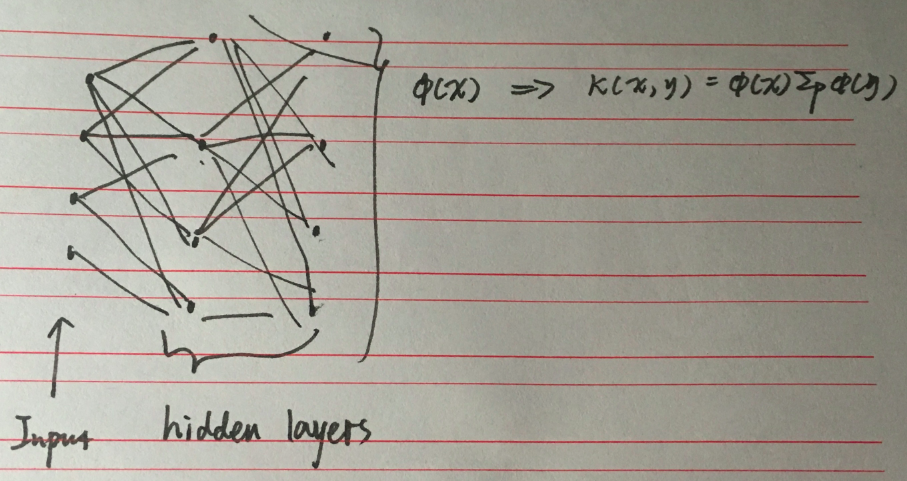
\includegraphics[width=\columnwidth]{./img/NN-GP.png}
    \caption{Architecture of the Gaussian process model with kernel characterized by deep neural network}
    \label{fig:NNGP}
\end{figure}

A Gaussian process model can also be derived from a feature-map view. Let $\phi(\bm{x}): R^D \rightarrow R^M$ be a feature map from $D$-dimensional input space to the $M$-dimensional feature space. We assume that the latent function $f(\bm{x})$ is a linear combination of the nonlinear features, and the observed target values are generated from $f(\bm{x})$ with addictive noise

\begin{equation}
    \label{eq:weightspace}
    \begin{array}{lll}
        f(\bm{x}) &=&    \bm{w}^T \phi(\bm{x})   \\
        y_i       &=&    f(\bm{x_i}) + \epsilon  \\
        \epsilon  &\sim& N(0, \sigma_n^2)
    \end{array}.
\end{equation}

If a zeros mean Gaussian prior with covariance matrix $\Sigma_p$ is imposed on the weights $\bm{w}$, i.e., $\bm{w} \sim N(0, \Sigma_p)$, it can be proved that $f$ follows a Gaussian process $f \sim \mathcal{GP}(0, k)$ \cite{GPML}, with the kernel function $k$ defined as
\begin{equation}
    \label{eq:kernel_from_weight}
    k(\bm{x}, \bm{y}) = \phi(\bm{x})^T \Sigma_p \phi(\bm{y}).
\end{equation}
The GP model defined from finite feature map is called \emph{degenerate} Gaussian process, as the covariance matrix calculated from \Fref{eq:kernel_from_weight} would have a lower rank $M$ than $N$.

%XXX: mension the matrix inversion lemma

If we set $\Sigma_p$ to a diagonal matrix $\Sigma_p = \frac{\sigma_p^2}{M} I$, the predictive distribution of \Fref{eq:GPRPred} can be re-formulated as
\begin{equation}
    \left\{
        \begin{array}{lll}
            \mu(\bm{x})      &= & \phi(x)^T A^{-1} \Phi \bm{y} \\
            \sigma^2(\bm{x}) &= & \sigma_n^2 + \sigma_n^2 \phi(\bm{x})^T A^{-1} \phi(\bm{x}) \\
            \Phi             &= & (\phi(\bm{x}_1),~\dots~,\phi(\bm{x}_N)) \\
            A                &= & \Phi \Phi^T + \frac{M \sigma_n^2}{\sigma_p^2} I
        \end{array}.
    \right.
    \label{eq:DegeneratePred}
\end{equation}

Note that the when calculating $\mu(\bm{x})$ and $\sigma^2(\bm{x})$ directly using \Fref{eq:GPRPred}, the time complexity are $O(N)$ and $O(N^2)$, respectively. However, if \Fref{eq:DegeneratePred} is used, the time complexity for calculating $\mu(\bm{x})$ and $\sigma^2(\bm{x})$ become $O(M)$ and $O(M^2)$ as long as the inverse of $A$ is pre-calculated.

The log likelihood of the training data defined in \Fref{eq:GPloglikelihood} can also be re-formulated as \cite{lazaro2010marginalized}
\begin{equation}
    \label{eq:DegenerateGPloglikelihood}
    \log p(\bm{y} | X, \bm{\theta}) = -\frac{1}{2\sigma_n^2}(\bm{y}^T\bm{y} - \bm{y}^T \Phi^T A^{-1} \Phi \bm{y}) - \frac{1}{2}\log |A| + \frac{M}{2} \log \frac{M \sigma_n^2}{\sigma_p^2} - \frac{N}{2} \log(2 \pi \sigma_n^2),
\end{equation}
where $\bm{\theta}$ is the vector containg $\sigma_p$, $\sigma_n$ and the parameters of $\phi$. In \Fref{eq:GPloglikelihood}, the covariance matrix $K$ should be inverted, which would take $O(N^3)$ operations. For \Fref{eq:DegenerateGPloglikelihood}, the matrix $A$ is of the size $M \times M$, so the time complexity for calculating \Fref{eq:DegenerateGPloglikelihood} is only $O(NM^2)$. Note that $M \ll N$.

% XXX: the loss function for the
It can be seen that GP model can be constructed from a finite feature map. Neural network (NN) can provide effective feature representations. It is thus naturally to use a neural network to approximate the feature map $\phi$. In \cite{lazaro2010marginalized}, a neural network with one hidden layer is proposed to approximate the feature map $\phi(\bm{x})$. The parameters of the neural network are obtained by maximizing the likelihood function in \Fref{eq:DegenerateGPloglikelihood} with gradient back-propagation. In \cite{huang2015scalable}, the single hidden layer is extended to multiple layers. The Gaussian process with kernel characterized by neural network is illustrated in \Fref{fig:NNGP}. A similar work is \cite{snoek2015scalable}, where a neural network is firstly pre-trained, and Bayesian linear regression is then performed to the last layer.

% \paragraph{Deep ensemble}
\subsection{Model Averaging to Improve the Quality of Uncertainty Prediction}\label{sec:deepensemble}

When probabilistic models are built from neural networks, a simple model averaging technique\cite{lazaro2010marginalized, huang2015scalable, lakshminarayanan2017simple} can significantly improve the quality of the estimated uncertainty.

Firstly, $K$ independent probabilistic neural network models are trained with random initializations. Each model would give predictive distribution $p(y | \bm{x}, \bm{\theta}_k) = N(\mu_k(\bm{x}), \sigma_k^2(\bm{x}))$ where $\bm{\theta}_k$ is the neural network parameters for the $k$-th model, $\mu_k(\bm{x})$ and $\sigma_k^2(\bm{x})$ are the mean and variance of the corresponding predictive Gaussian distribution. The final predictive distribution can be expressed as $p(y | \bm{x}) = N(\mu(\bm{x}), \sigma^2(\bm{x})$, where
\begin{equation}
    \left\{
        \begin{array}{lll}
            \mu(\bm{x})      &=& \frac{1}{K} \sum_k \mu_k(\bm{x}) \\
            \sigma^2(\bm{x}) &=& \frac{1}{K} \sum_k (\mu_k^2(\bm{x}) + \sigma_k^2(\bm{x})) - \mu^2(\bm{x})
        \end{array}.
    \right.
    \label{eq:deepensemble}
\end{equation}

In \cite{lazaro2010marginalized, huang2015scalable}, the uncertainty is obtained according to \Fref{eq:DegeneratePred}. However, in \cite{lakshminarayanan2017simple}, the uncertainty is generated by adversarial training. It is shown that the ensemble technique defined in \Fref{eq:deepensemble} can greatly improve the quality of the uncertainty measure. In \cite{lakshminarayanan2017simple}, with $K = 5$, the model-averaging significantly improves the quality of the uncertainty estimation, and outperforms Bayesian-based models like probabilistic backpropagation \cite{hernandez2015probabilistic} and MC-dropout \cite{gal2016dropout}.
